\subsection{Improving the baseline}

\subsubsection{Symmetric strategies}
Following these results, we can wonder how to improve the efficiency of the simple V-cycle with 1 relaxation step.
The first step is to analyze the time spent in the different parts of a cycle. All the different matrices $A$ for each level are computed in a setup phase so we do not need to analyze these computation times. We only focus on measuring these two different computations: (i) the time spent doing a relaxation at each level and (ii) the time spent computing the next linear system
(when going down in the grid), i.e. restricting the solution to a coarser grid, which is a sparse matrix-vector computation or the time spent interpolating the error term (when going up in the grid) which is another sparse matrix-vector computation. The values where measured for a problem (an unstructured domain with some anisotropy, denoted by Unstructed-Anisotropy) of size 512000 with a 8-level grid and are presented
in Table~\ref{table.measures}, along with some information on the matrix used at the corresponding level.

\begin{table}
  \resizebox{\linewidth}{!}{
 \begin{tabular}{|c|c|c|c|c|c|c|}
 \hline
 Level & Matrix size & Non-zero & Relax (down) & Relax (up) & Matvec (down) & Matvec (up) \\
 \hline
  1 & 512,000 & 4,042,520 & 20 ms & 20 ms & 15 ms & -\\
 \hline
  2 & 256,000 & 6,475,239 & 20 ms & 25 ms & 12 ms & 4 ms\\
 \hline
  3 & 58,893 & 2,000,513 & 8 ms & 8 ms & 3 ms & 2 ms\\
 \hline
  4 & 14,285 & 788,509 & 2 ms & 2 ms & 1 ms & 0.7 ms\\
 \hline
  5 & 4,238 & 386,333 & 1 ms & 1 ms & 0.5 ms & 0.2 ms\\
 \hline
  6 & 609 & 53,493 & 0 ms & 0 ms & 0 ms & 0 ms\\
 \hline
  7 & 69 & 2,873 & 0 ms & 0 ms & 0 ms & 0 ms\\
 \hline
  8 & 2 & 4 & 0 ms & - & - & 0 ms\\
 \hline
 \end{tabular}
 }
 \caption{Approximate times spent in the different parts of a V-cycle with $\alpha=1$.}
 \label{table.measures}
\end{table}
 In practice, we notice that the number of non-zero entries in the input matrix is correlated to the average time of a relaxation at a given level. Most importantly, in this example we see that, overall,
 the relaxation represents $\approx66\%$ of the total cost of a V-cycle (while the matrix-vector multiplications are only $\approx30\%$) and that the two first levels are from far the most expensive ones.
 With this information, there are two ideas: (i) adding more relaxations in the last levels because it is almost free or (ii) removing some relaxations in the first levels to reduce the computational cost.
 
 The following 4 strategies were then tested on this same matrix.
  \begin{itemize}
   \item \emph{Fast} : no relaxation at level 2.
   \item \emph{Fast4} : no relaxation at level 3.
   \item \emph{Fast2} : 10 relaxations at level $L-2$.
   \item \emph{Fast3} : 2 relaxations at levels $L-2,L-4,\dots,3$.
  \end{itemize}
  The strategy \emph{Fast} aims at reducing the cost of the cycle by removing the penultimate relaxation (hoping the accuracy lost at this point will be compensated by the relaxation at level 0) which is very costly.
  The strategy \emph{Fast4} is a softer version of \emph{Fast} where the relaxation at level 3 is removed, reaching less improvement of the overall execution time but being more easily compensated by the two relaxations at level 1 and 2.\\
  The strategy \emph{Fast2} executes a lot of relaxations at level $L-2$, because it should not increase by much the execution time of the V-cycle. Why choose $L-2$ level instead of $L$ or $L-1$?
  This because the relaxation at level $L$ is actually a direct solve. Thus, the error term is almost exact at level $L-1$, because the only source of error
  comes from the interpolation of $e^L$ (which is exact) into $e^{L-1}$. This is why, we might expect better results by adding relaxations at level $L-2$.
  The last strategy \emph{Fast3}, pushes this idea one step further. If we assume that doing more than one relaxation gets a really accurate error estimation at level $l$, then
  at level $l-1$ we do not need to correct a lot by doing more relaxations. However at level $l-2$ we have been through 2 interpolations since last good estimation of the error vector, hence increasing the number of relaxations again.
  As we still want not to increase the execution time a lot we stop this recursion for the first levels as they are the two most costly relaxations.
  
  \begin{figure}
  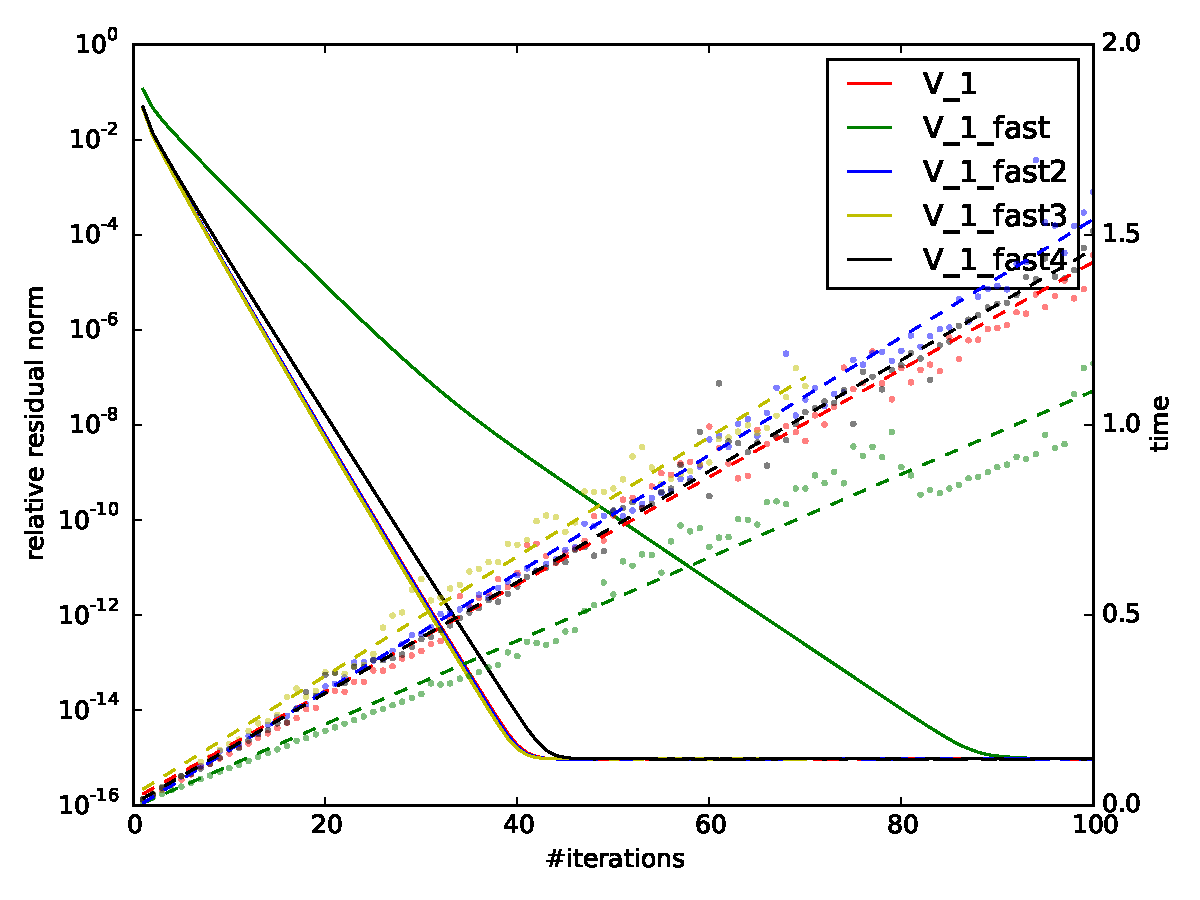
\includegraphics[width=0.49\linewidth]{figs/convergence_fast_small.pdf}
   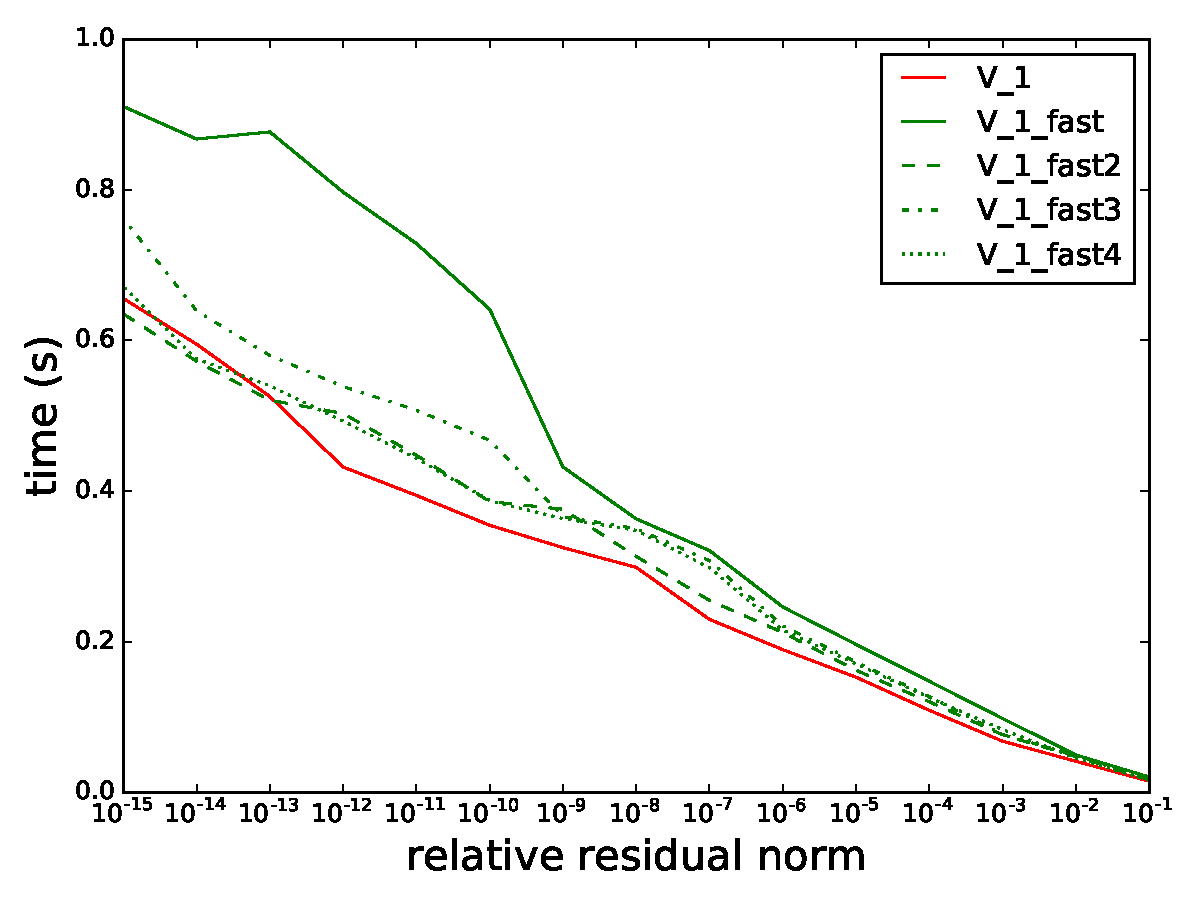
\includegraphics[width=0.49\linewidth]{figs/time_convergence_fast_small.pdf}
   \caption{Execution time and final residual norm for the 4 new strategies on a small matrix.}
   \label{fig.newstrat_small}
  \end{figure}

  In Figure~\ref{fig.newstrat_small}, we present the results of these 4 strategies on a smaller matrix of initial size 64,000 with only a 6-level grid.
  The first thing to observe is that removing the relaxation at level 1 does not provide any benefit. It sure saves time during a cycle but the accuracy loss is tremendous.
  The other thing to notice is that adding a lot of relaxations in the last levels increases by a little the execution time while being useless on the accuracy side. This is why \emph{Fast2} and  \emph{Fast3} are not really efficient.
  
  More tests were performed on the original $512,000\times 512,000$ matrix and are presented in Figure~\ref{fig.newstrat}.
  
  \begin{figure}
  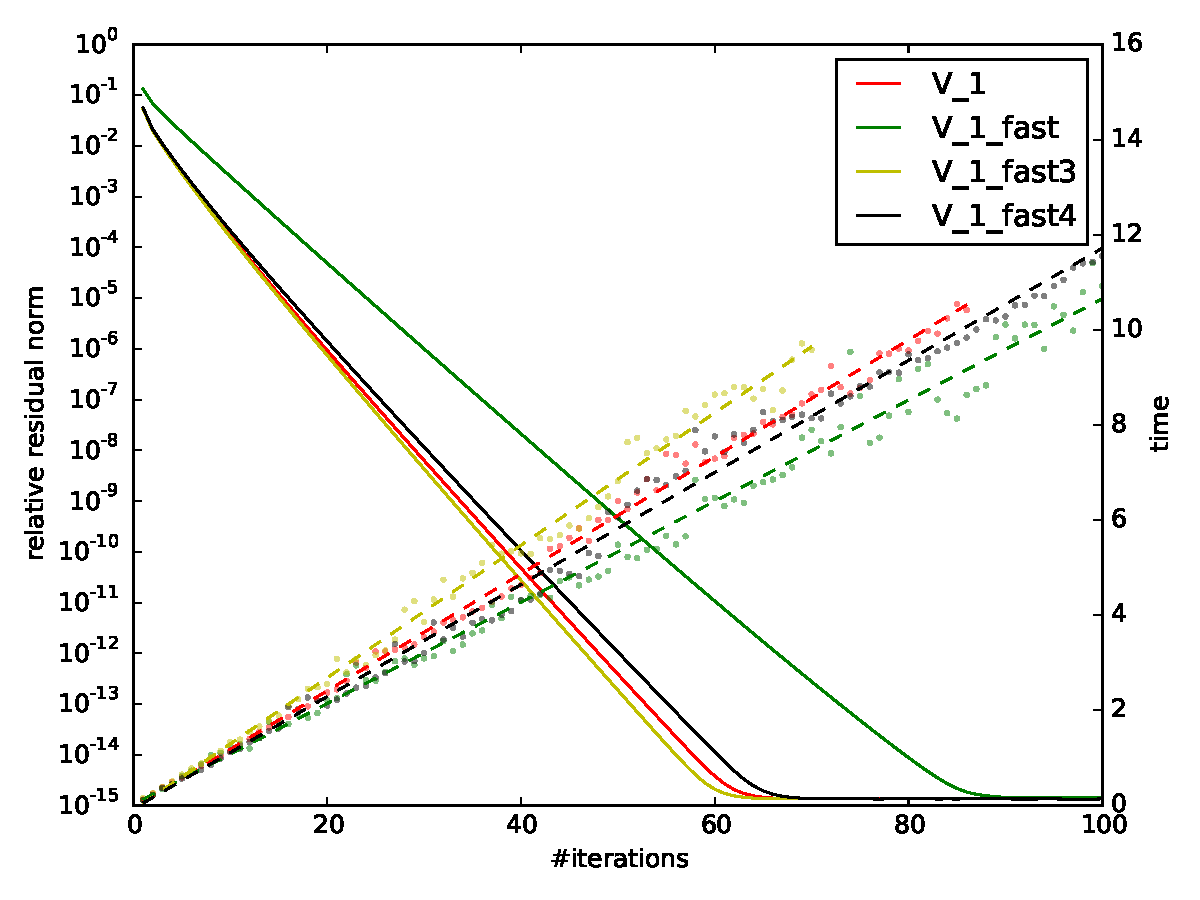
\includegraphics[width=0.49\linewidth]{figs/convergence_fast.pdf}
   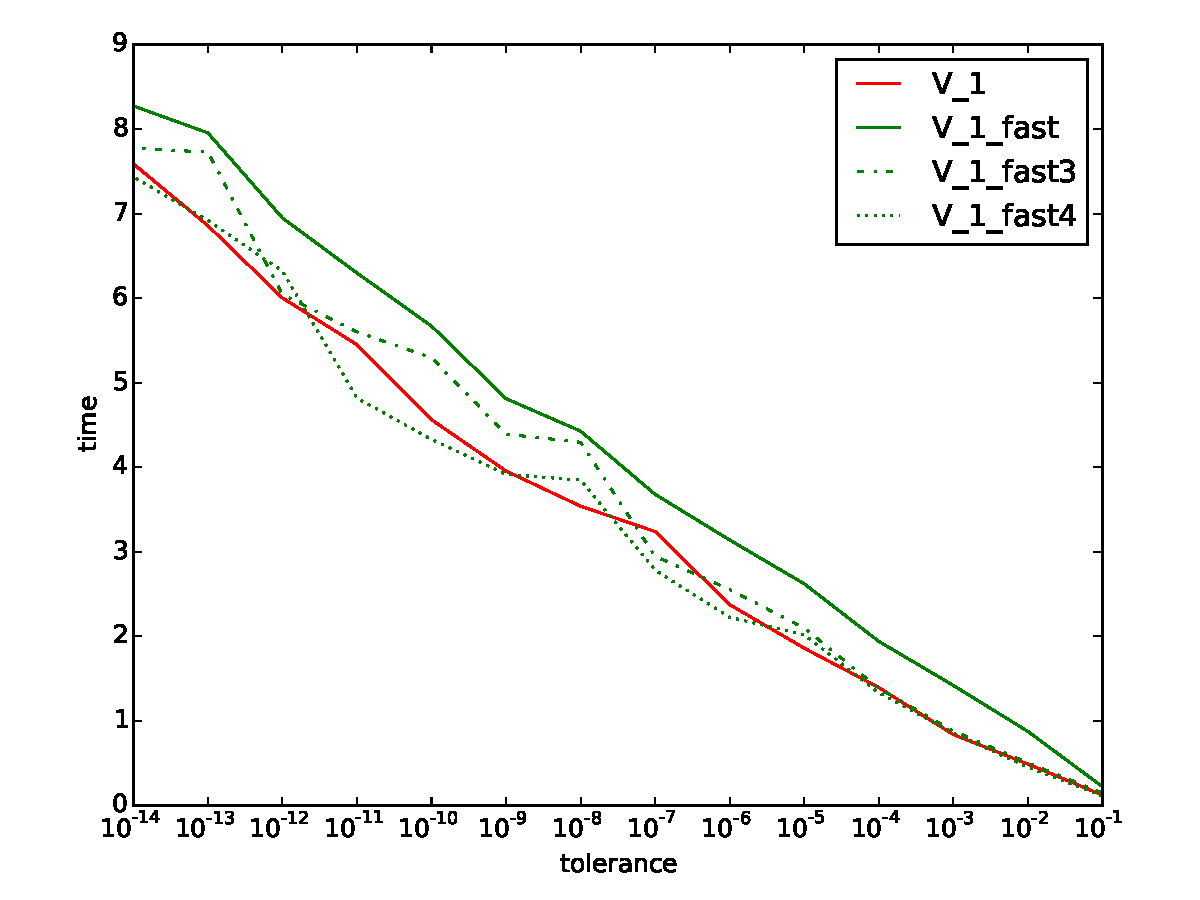
\includegraphics[width=0.49\linewidth]{figs/time_convergence_fast.pdf}
   \caption{Execution time and final residual norm for the 4 new strategies on the bigger matrix.}
   \label{fig.newstrat}
  \end{figure}
  
\subsubsection{An asymmetric strategy}
\label{sec.assymetric}
  We observe no big improvement compared to the original V-cycle with 1 relaxation at each level with the previous strategies.
  Their common point is that they all do the same number of relaxations when going down or up in the cycle. However, the main idea of the multi-grid algorithm is totally asymmetric: the relaxations before
going to a coarser level is there to compute a first approximate solution to the current system while the relaxations before going back to a finer level are here to refine the error term.
  We first compute an approximation at a given level $l$, then we use the level $l+1$ to compute an approximate error term $e^l$ and finally we redo some relaxation to refine the solution. The two relaxations do not have the same goal.
  What if we could ensure that any value of the error vectors will be less than $\epsilon$ from the exact value just by doing a relaxation step? We would not need to do a relaxation
  before computing the approximate error term using the next levels in the grid but compute directly the error term when we go back up in the cycle. From that idea we define a new asymmetric strategy: we use a V-cycle with $\alpha_1 = 0$ and $\alpha_2 = 1$. In other words
  we do one relaxation at each level only when we are going up in the cycle. We call this strategy \emph{Up}.
  
  We run \emph{Up} and \emph{Fast4}, as long as the classical V-cycle, on the same matrix of size 512,000 and also on
  other applications (3D laplace with a 9-pt stencil, 3D laplace with a 27-point stencil, and another 3D partial derivative equation with Dirichlet boundary conditions) with the same size of matrix.
  
  All results are presented in Figure~\ref{fig.up_comparison}.
  
  \begin{figure}
   \subfloat[\textsc{Unstructured-Anisotropy}]{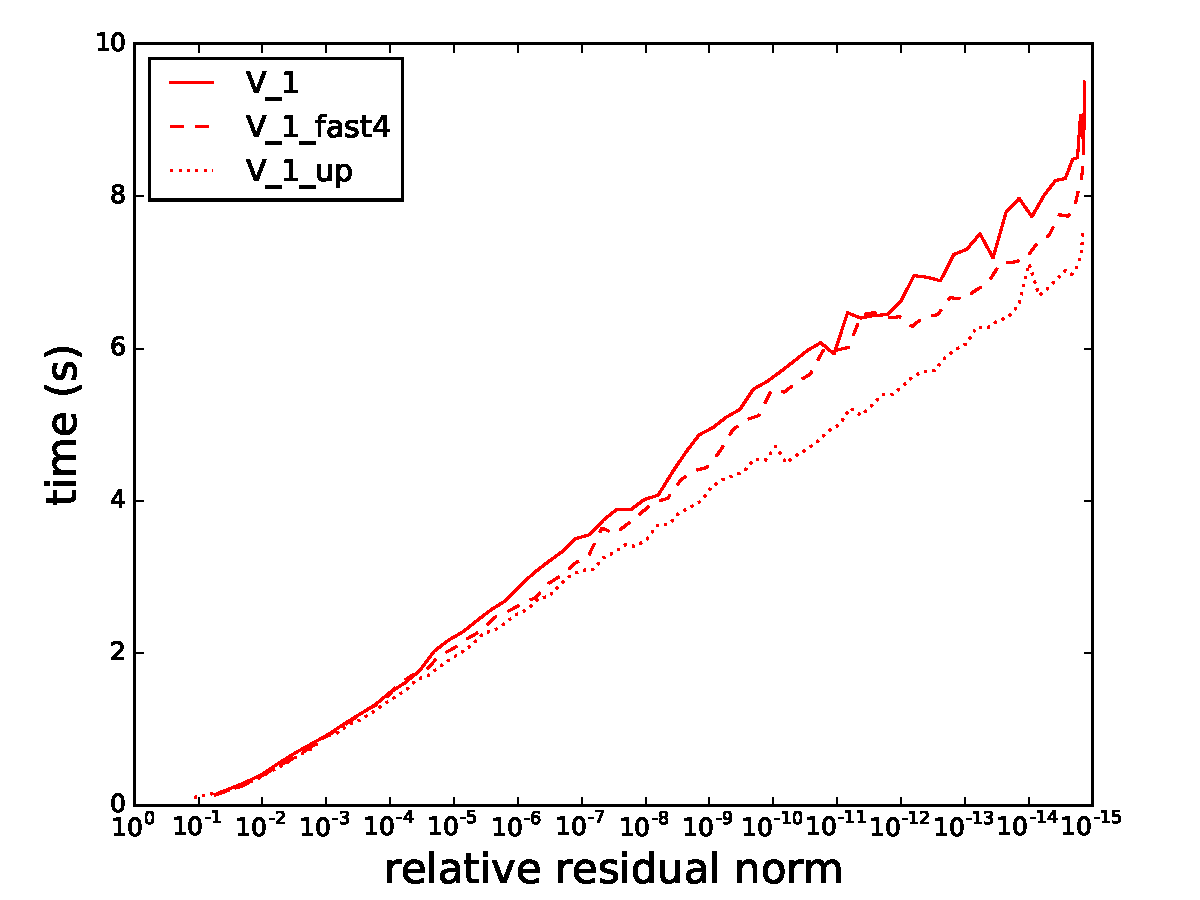
\includegraphics[width=0.49\linewidth]{figs/time_convergence_up_1.pdf}}
   \subfloat[\textsc{3DLaplace-9pt}]{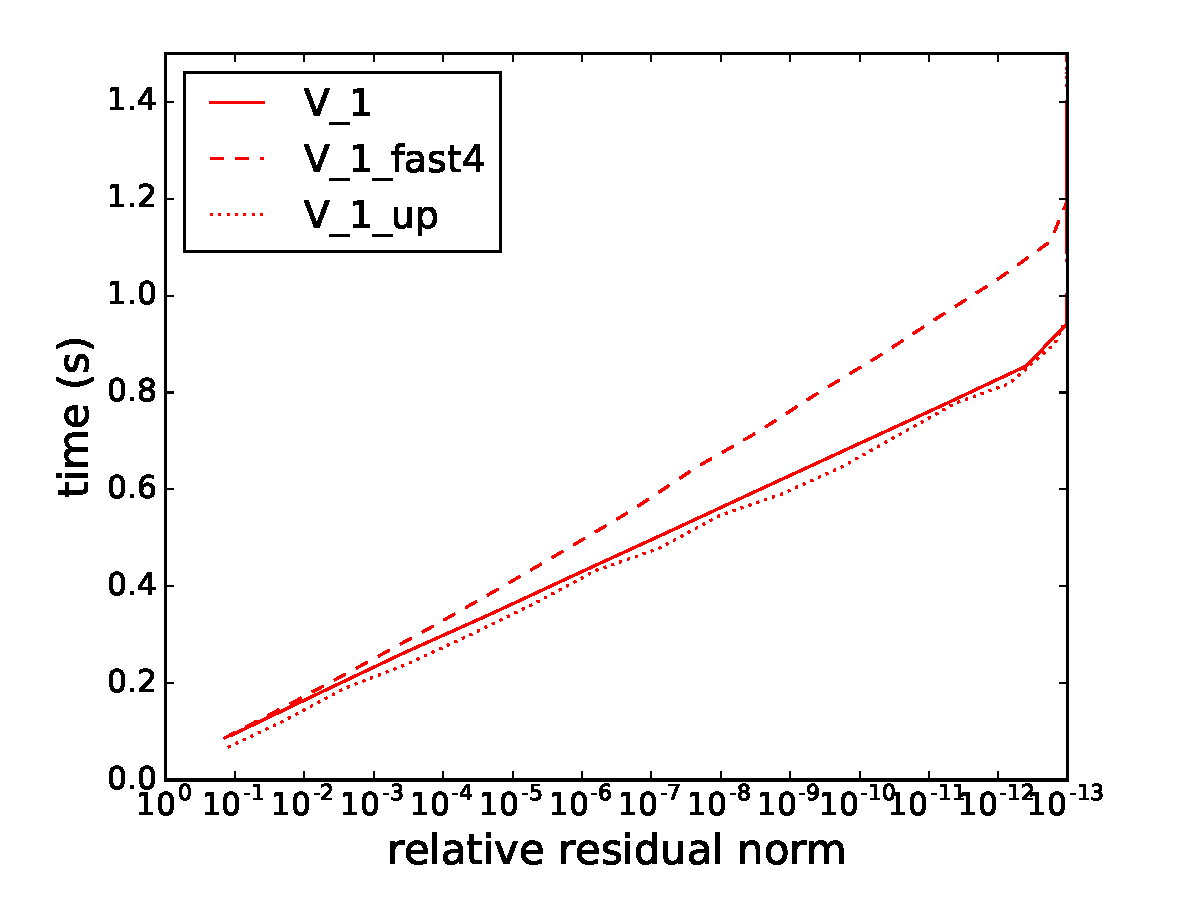
\includegraphics[width=0.49\linewidth]{figs/time_convergence_up_2.pdf}}\\
   \subfloat[\textsc{3DLaplace-27pt}]{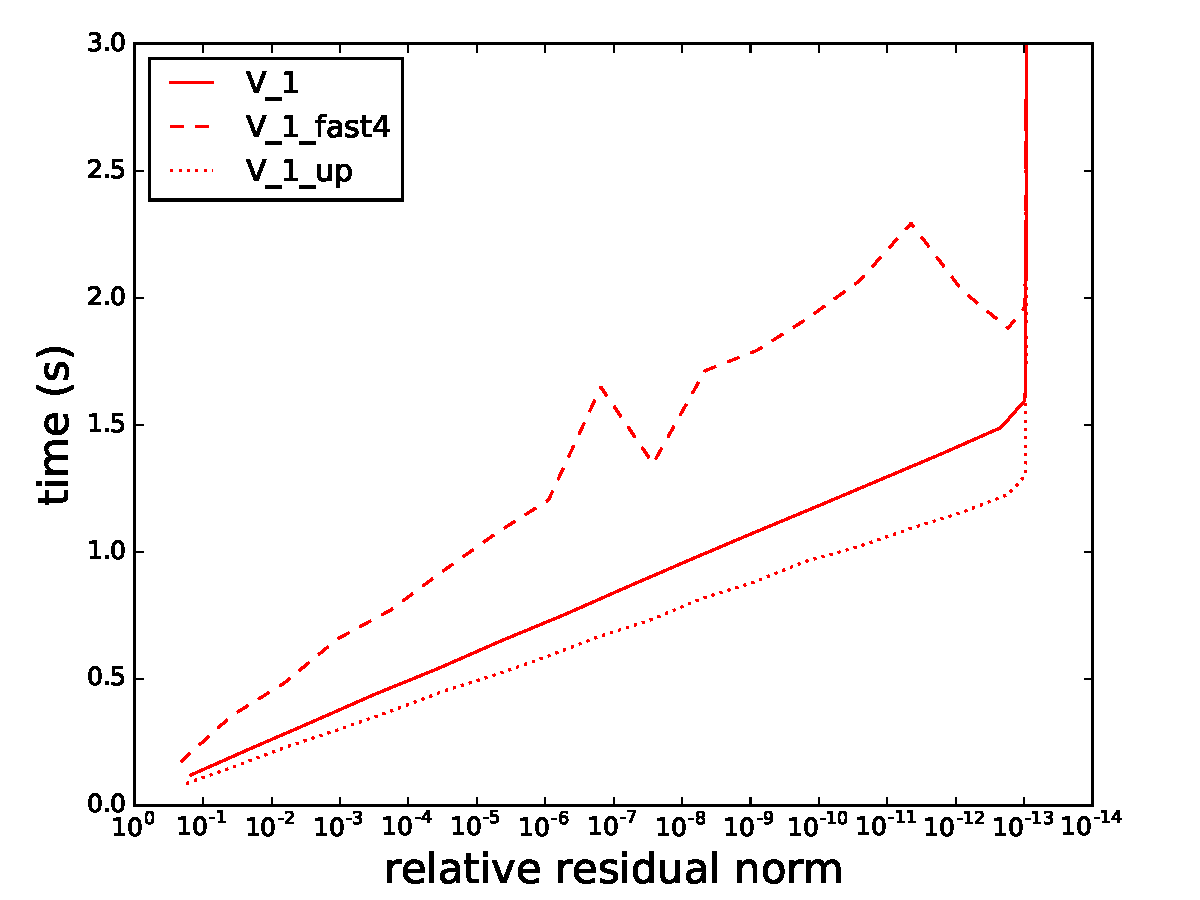
\includegraphics[width=0.49\linewidth]{figs/time_convergence_up_3.pdf}}
   \subfloat[\textsc{PDE-Dirichlet}]{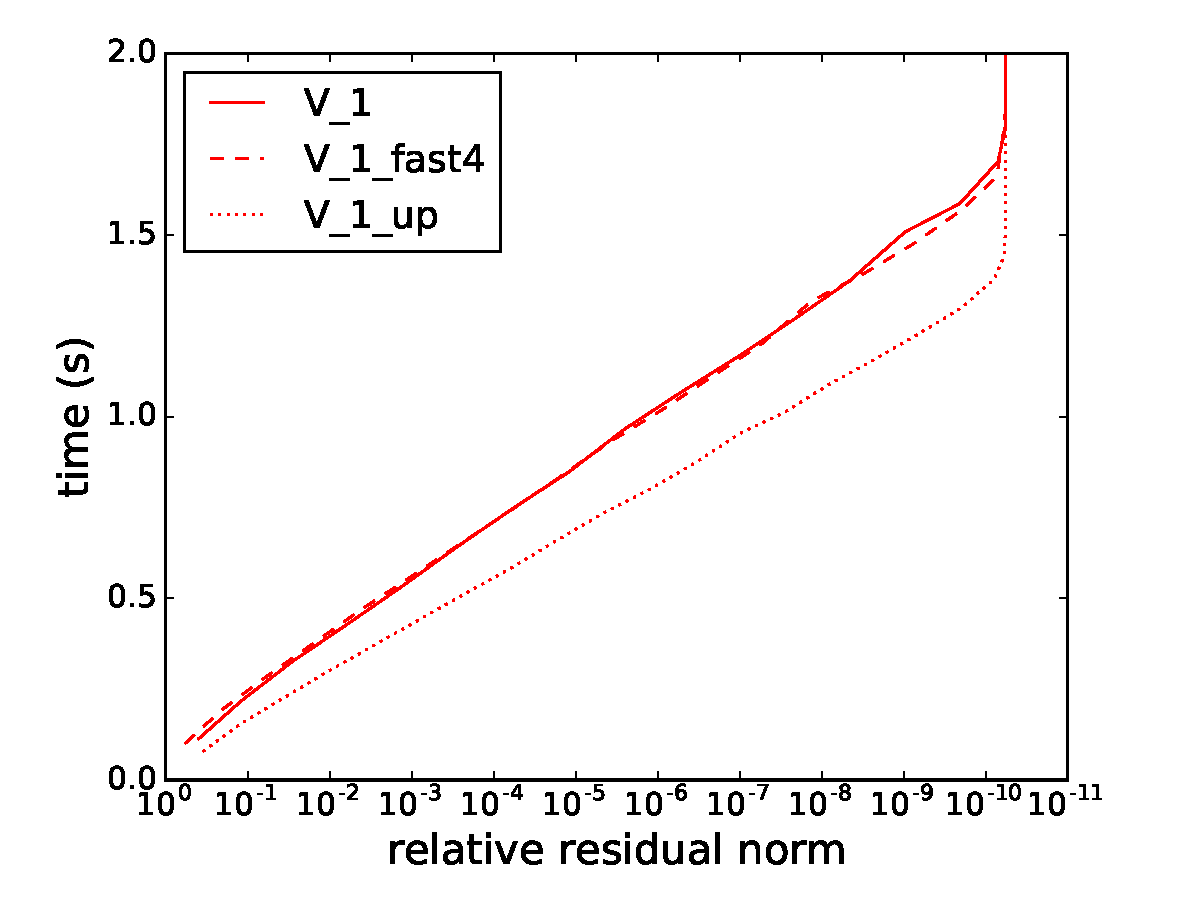
\includegraphics[width=0.49\linewidth]{figs/time_convergence_up_4.pdf}}
   \caption{Comparison of original algorithm with \emph{Fast4} and \emph{Up} strategies.}
   \label{fig.up_comparison}
  \end{figure}

   At this point, we see that it is not worth considering the \emph{Fast4} strategy anymore. However, \emph{Up} seems to be
   quite efficient since it improves by $12\%$,$7\%$,$20\%$ and $22\%$ (for \textsc{Unstructured-Anisotropy}, \textsc{3DLaplace-9pt}, \textsc{3DLaplace-27pt} and \textsc{PDE-Dirichlet} respectively) the average time needed to reach
   a $10^{-i}$ precision.
   However all these runs are sequential and does not guarantee the viability of the \emph{Up} strategy when the algorithm is parallelized.
   More tests were performed on MinoTauro with bigger matrices and different processor topologies. The total size of the matrix is set to either
   5,832,000 or 13,824,000, while the topology will be composed of either 27 (3x3x3), 36 (6x6x1) or 64 (4x4x4) processors, where each processor holds 1 MPI process and there is only 1 OpenMP thread per process.
   The problems tested were \textsc{3DLaplace-9pt} and \textsc{3DLaplace-27pt}.
   For these 6 possible combinations, we observe an averaged improvement of 18.4\% (ranging from 16.0\% to 28.3\%) for \textsc{3DLaplace-9pt} and 20.5\% (ranging from 16.2\% to 25.0\%) for \textsc{3DLaplace-27pt}. It seems that \emph{Up} outperforms
   even more the classical V-cycle when the problem size increases, but seems to cap at around 25\% improvement. Figure~\ref{fig.mtup} presents the results for the matrix size 13,824,000 and \textsc{3DLaplace-27pt}, for the 3 different processor topologies. We have similar figures
   for the other scenarios.
   
   \begin{figure*}[t]
    \subfloat[3x3x3]{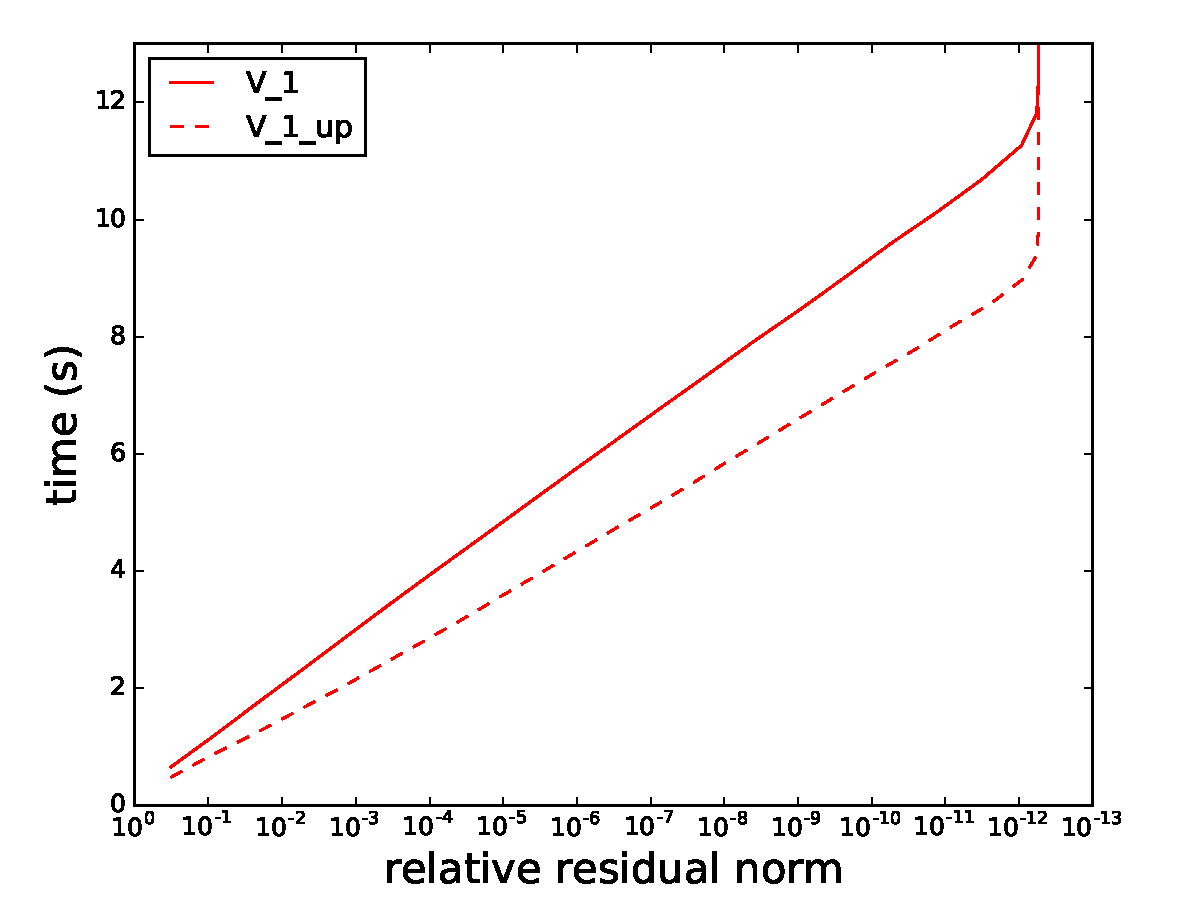
\includegraphics[width=0.33\linewidth]{figs/mt_27.pdf}}
    \subfloat[4x4x4]{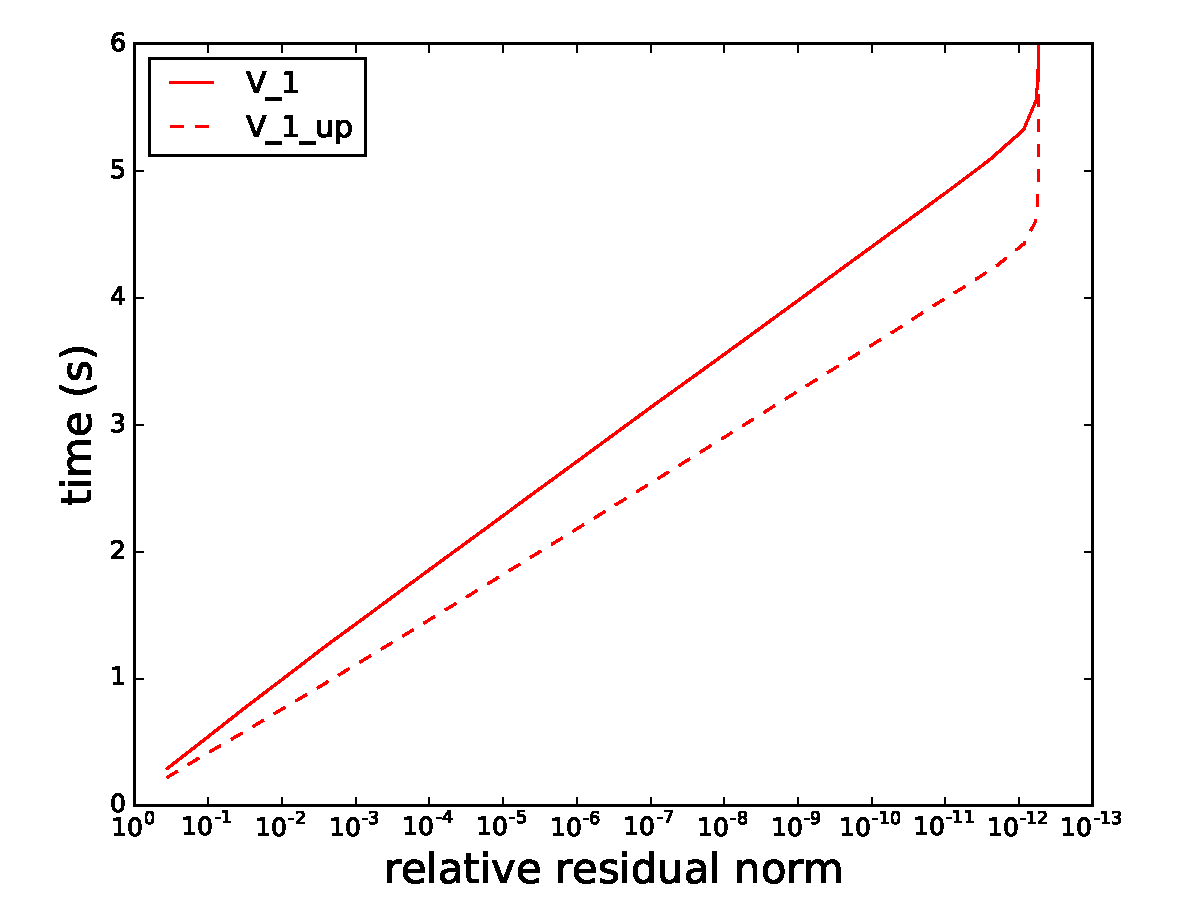
\includegraphics[width=0.33\linewidth]{figs/mt_64.pdf}}
    \subfloat[6x6x1]{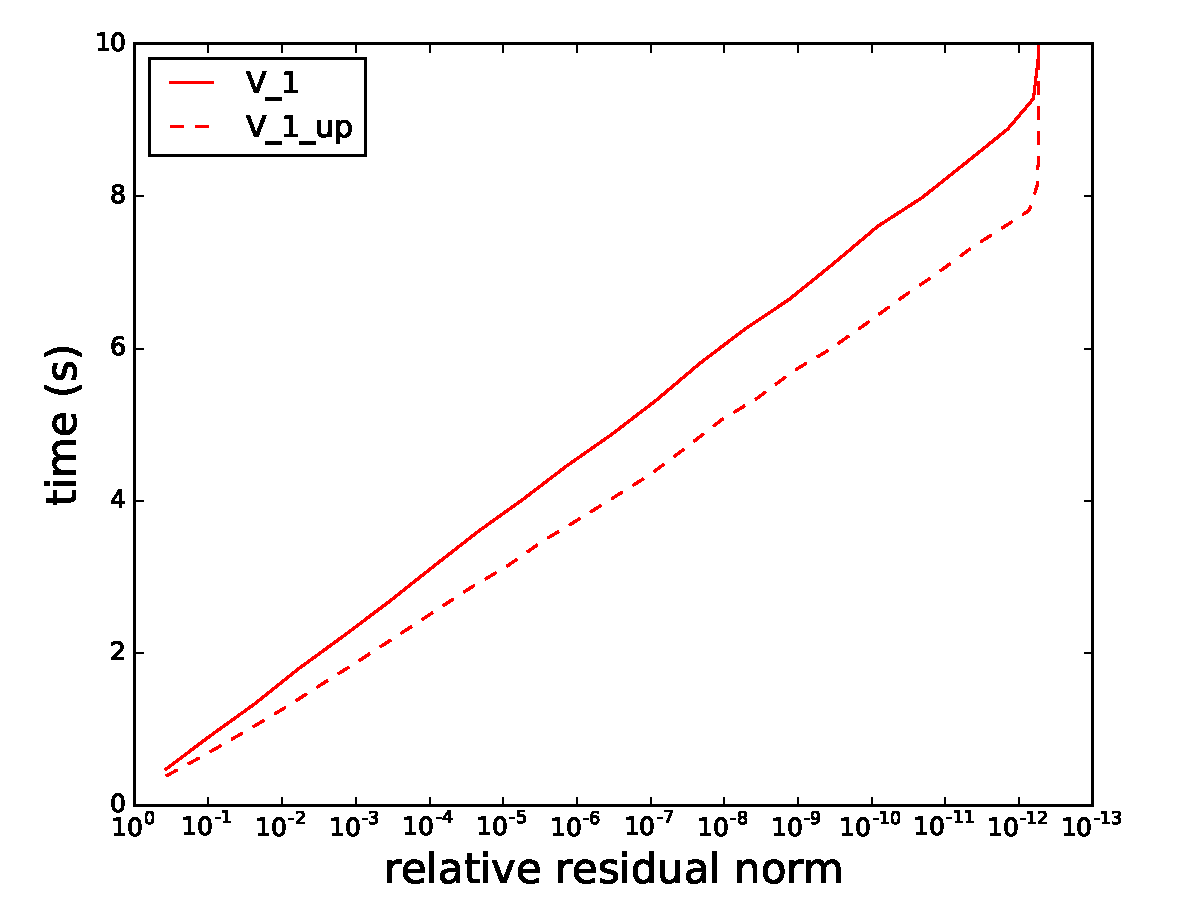
\includegraphics[width=0.33\linewidth]{figs/mt_36.pdf}}
    \caption{Comparison of original algorithm with \emph{Up} strategy for \textsc{3DLaplace-27pt} on a 240x240x240 grid.}
    \label{fig.mtup}
   \end{figure*}
